%%%%%%%%%%%%%%%%%%%%%%%%%%%%%%%%%%%%%%%%%%%%%%%%%%%%%%%%%%%%%%%%%
%%% %
%%% % weiiszablon.tex
%%% % The Faculty of Electrical and Computer Engineering
%%% % Rzeszow University Of Technology diploma thesis Template
%%% % Szablon pracy dyplomowej Wydziału Elektrotechniki 
%%% % i Informatyki PRz
%%% % June, 2015
%%%%%%%%%%%%%%%%%%%%%%%%%%%%%%%%%%%%%%%%%%%%%%%%%%%%%%%%%%%%%%%%%

\documentclass[12pt,twoside]{article}

\usepackage{weiiszablon}

\author{}

% np. EF-123456, EN-654321, ...
\studentID{PL-167800}

\title{Realizacja sieci neuronowej uczonej algorytmem wstecznej propagacji błędu, uczącą się diagnozowania chorób}
\titleEN{Temat pracy po angielsku}


%%% wybierz rodzaj pracy wpisując jeden z poniższych numerów: ...
% 1 = inżynierska	% BSc
% 2 = magisterska	% MSc
% 3 = doktorska		% PhD
%%% na miejsce zera w linijce poniżej
\newcommand{\rodzajPracyNo}{0}


%%% promotor
\supervisor{dr hab. inż. Roman Zajdel, prof. PRz}
%% przykład: dr hab. inż. Józef Nowak, prof. PRz

%%% promotor ze stopniami naukowymi po angielsku
\supervisorEN{(academic degree) Imię i nazwisko opiekuna}

\abstract{Treść streszczenia po polsku}
\abstractEN{Treść streszczenia po angielsku}

\begin{document}

% strona tytułowa
\maketitle

\blankpage

% spis treści
\tableofcontents

\clearpage
\blankpage

\section{Wstęp}
\subsection{Cel projektu}

Głównym założeniem projektu jest realizacja sieci neuronowej uczonej za pomocą algorytmu wstecznej propagacji błędu, której zadaniem jest zdiagnowanie choroby piersi na podstawie pewnych danych wejściowych.
W ramach projektu zbadano wpływ poszczególnych parametrów sieci na proces jej uczenia:
\begin{itemize}
	\item S1 - ilość neuronów w I warstwy ukrytej
	\item S2 - ilość neuronów w II warstwy ukrytej
	\item lr (learning rate) / eta - wartość współczynnika uczenia
\end{itemize}
Jako zbiór danych uczących wykorzystano zbiór „Breast Tissue”, a sama sieć została zrealizowana przy użyciu języka programowania Python.
\newpage
\subsection{Opis problemu}
Realizowana sieć na podstawie podanych informacji wejściowych ma za zadanie sklasyfikować, do której klasy należą te dane i na wyjściu podać informacje o rodzaju zdiagnowzowanej choroby.
W zbiorze danych uczących występuje 6 możliwych klas:
\begin{itemize}
	\item car (carcinoma) - rak
	\item fad (fibro-adenoma) - gruczolakowłókniak, czyli łagodny nowotwór piersi
	\item mas (mastopathy) - chorobia sutka
	\item gla (glandular) - gruczolakorak
	\item con (connective) - choroba tkanki łącznej
	\item adi (adipose) - choroba tkanki tłuszczowej
\end{itemize}
Na rysunku~\ref{Fig:rozklad_klas_proc} pokazano procentowy, a na rysunku~\ref{Fig:rozklad_klas_ilosc} ilościowy rozkład klas w zbiorze:
\begin{figure}[ht!]
	\centering
	\includegraphics[]{figures/rozklad_klas_proc.png}
	\caption{Procentowy rozkład klas w zbiorze}
	\label{Fig:rozklad_klas_proc}
\end{figure}
\begin{figure}[ht!]
	\centering
	\includegraphics[]{figures/rozklad_klas_ilosc.png}
	\caption{Ilościowy rozkład klas w zbiorze}
	\label{Fig:rozklad_klas_ilosc}
\end{figure}
\newpage
\subsection{Opis zestawu danych}
Zestaw danych uczących został pobrany ze strony:

\url{https://archive.ics.uci.edu/ml/datasets/Breast+Tissue}

Zbiór danych uczących zawiera 106 rekordów z 6-ciu klas zawierającymi po 10 atrybutów w każdym wierszu.
W przypadku atrybutów, będących parametrami wejściowymi są to:
\begin{itemize}
	\item I0 - Impedancja (om) przy zerowej częstotliwości
	\item PA500 - kąt fazowy przy 500 KHz
	\item HFS - nachylenie wysokiej częstotliwości kąta fazowego
	\item DA - odległość impedancji między końcami widmowymi
	\item AREA - obszar pod widmem
	\item A/DA - obszar znormalizowany przez DA
	\item MAX IP - maksimum widma
	\item DR - odległość między I0 a rzeczywistą częścią punktu maksymalnej częstotliwości
	\item P - długość krzywej widmowej
\end{itemize}
\newpage
\subsection{Przygotowanie danych}
Badany zestaw danych nie zawiera niekompletnych rekordów, oraz wartości niepoprawnych, dlatego też podczas przygotowywania danych nie napotkano żadnych nieprzewidzianych błędów.

W celu ujednolicenia danych do poźniejszego przetwarzania na danych przeprowadzono normalizację zgodnie z poniższym wzorem:
\begin{equation}
	x_{norm}=\frac{x-x_{min}}{x_{max}-x_{min}}
	\label{Eq:normalizacja}
\end{equation}
gdzie:
\begin{itemize}
	\setlength\itemsep{0em}
	\item $x_{norm}$ - wartość po normalizacji
	\item $x$ - wartośc przed normalizacją
	\item $x_{min}$ - minimalna wartość w zbiorze
	\item $x_{max}$ – maksymalna wartość w zbiorze
\end{itemize}
Dzięki zastosowaniu wzoru~\ref{Eq:normalizacja} pierwotne dane wejściowe każdego rekordu zostały zamienione na odpowiadające im wartości z zakresu od 0 do 1.
\newpage
\section{Zagadnienia teoretyczne}
\subsection{Model sztucznego neuronu}
Każda sieć neuronowa składa się z połączonych między sobą pojedynczych neuronów. Należy zatem zapoznać się z modelem pojedynczego neuronu w celu zrozumienia problemu sieci neuronowych. Przykładowy model pojedynczego neuronu został przedstawiony na rysunku~\ref{Fig:neuron}
\begin{figure}[ht!]
	\centering
	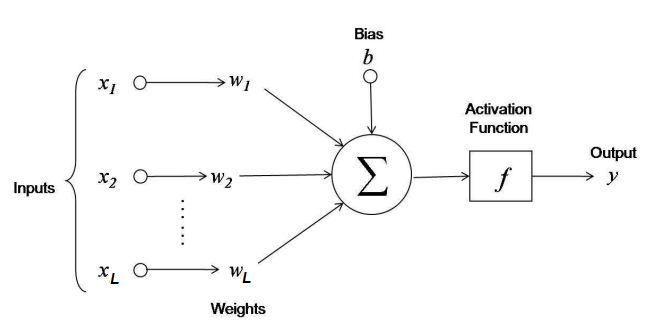
\includegraphics[width=12cm]{figures/model_neuronu.png}
	\caption{Model pojedynczego neuronu}
	\label{Fig:neuron}
\end{figure}

Każdy neuron to układ składający się z wielu wejść i jednego wyjścia. Wszystkie wejścia posiadają tzw. współczynnik wagowy, który określa jak bardzo dane wejście wpływa na rezultat wynikowy danego neuronu. Oprócz wagi dodatkowym elementem wejściowych jest również bias, umożliwiający przesunięcie funkcji aktywacji w lewo lub w prawo danego neuronu.
Całość z poprzednio podanych informacji do wejść neuronu trafia do sumatora gdzie odbywa się proces wyznaczania łącznego pobudzenia
neuronu, wyrażanego z następującego wzoru~\ref{Eq:pobudzenie}:
\begin{equation}
	z = \sum_{j=1}^{L} w_{j}x_{j}+b
	\label{Eq:pobudzenie}
\end{equation}
Wyznaczona wartość następnie trafia do funkcji aktywacji, gdzie określany jest sygnał wyjściowy neuronu zgodnie z zależnością \ref{Eq:aktywacja}:
\newpage
\begin{equation}
	y = f(z) = f(\sum_{j=1}^{L} w_{j}x_{j}+b)
	\label{Eq:aktywacja}
\end{equation}
gdzie:
\begin{itemize}
	\item $y$ - wyjście neuronu
	\item $x_{j}$ - \textit{j}-ty sygnał wejściowy (\textit{j=1,2,\dots,L})
	\item $w_{j}$ - waga \textit{j}-tego wejścia
	\item $b$ - bias
\end{itemize}
\subsection{Funkcja aktywacji}
Każda warstwa w swoich neuronach może wykorzystywać inną funkcję aktywacji.
W przypadku sieci jednokierunkowych najbardziej powszechna jest funkcja sigmoidalna, w której wyróżnić można dwa typy:
\begin{itemize}
	\item unipolarna funkcja aktywacji, która przyjmuje wartości w przedziału (0,1):
\end{itemize}
\begin{equation}
	f(x) = \frac{1}{1+e^{-x}}
	\label{Eq:unipolar_sigmoid}
\end{equation}
\begin{itemize}[resume]
	\item bipolarna funkcja aktywacji, przyjmująca wartości z przedziału (-1,1):
\end{itemize}
\begin{equation}
	f(x) = \frac{2}{1+e^{-x}} - 1
	\label{Eq:bipolar_sigmoid}
\end{equation}
Funkcje te są różniczkowalne i ich pochodne wyrazić można jako:
\begin{itemize}
	\item w przypadku unipolarnej funkcji aktywacji:
\end{itemize}
\begin{equation}
	f(x) = \frac{1}{1+e^{-x}}(1-\frac{1}{1+e^{-x}})
	\label{Eq:unipolar_sigmoid_pochodna}
\end{equation}
\begin{itemize}[resume]
	\item w przypadku bipolarnej funkcji aktywacji:
\end{itemize}
\begin{equation}
	f(x) = 1 - (\frac{2}{1+e^{-x}})^2
	\label{Eq:bipolar_sigmoid_pochodna}
\end{equation}
\newpage
\subsection{Model sieci jednokierunkowej wielowarstwowej}
W każdej sieci jednokierunkowej wielowarstwowej wyróżnić można nastepujące warstwy: wejścia, wyścia i występujące pomiędzy nimi warstwy ukryte.
W przypadku sieci jednokierunkowej dane mogą przepływać tylko w jednym kierunku od warstwy wejścia do warstwy wyjścia.
\begin{figure}[ht!]
	\centering
	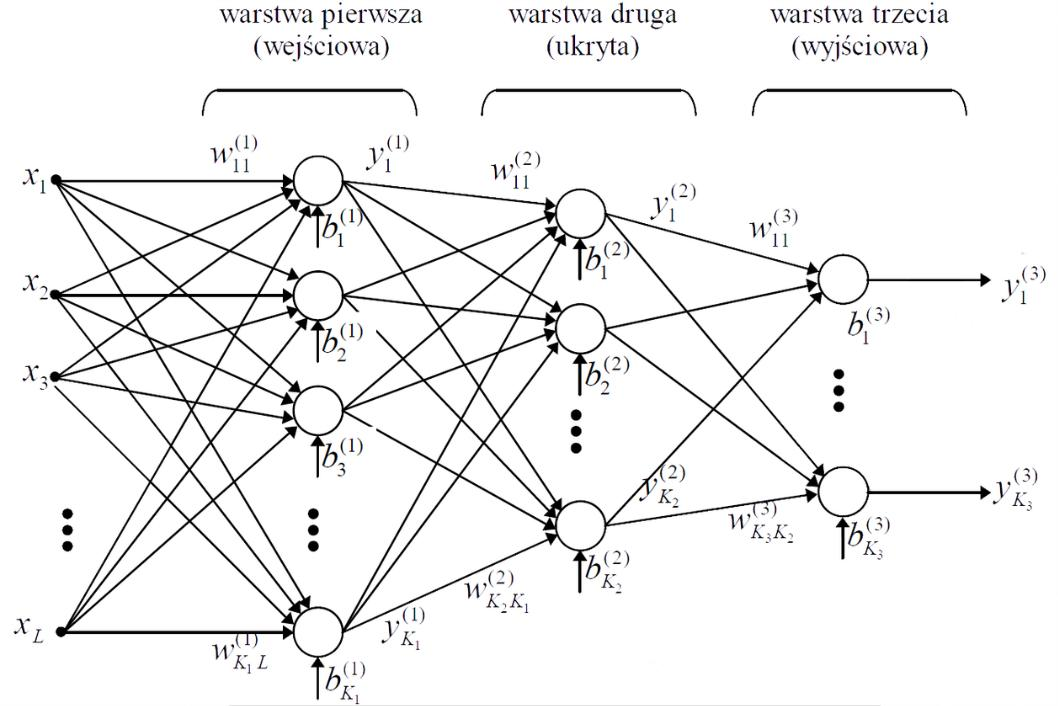
\includegraphics[width=12cm]{figures/model_sieci.png}
	\caption{Model sieci jednokierunkowej wielowarstwowej}
	\label{Fig:model_sieci}
\end{figure}

Każda pojedyncza warstwa neuronów posiada:
\begin{itemize}
	\item macierz wag \textbf{w}:
\end{itemize}
\begin{equation*}
	w =
	\begin{bmatrix}
		w_{11} & w_{12} & \dots & w_{1L}\\
		w_{21} & w_{22} & \dots & w_{2L}\\
		\vdots & \vdots &  & \vdots\\
		w_{K1} & w_{K2} & \dots & w_{KL}
	\end{bmatrix}
\end{equation*}
gdzie:
\begin{itemize}[resume]
	\begin{itemize}
		\item $K$ – liczbę neuronów w warstwie
		\item $L$ – liczba sygnałów wejściowych
	\end{itemize}
	\item wektor przesunieć \textbf{b}:
\end{itemize}
\begin{equation*}
	b =
	\begin{bmatrix}
		b_{1} & b_{2} & \dots & b_{K}
	\end{bmatrix}^{T}
\end{equation*}
\begin{itemize}[resume]
	\item funkcje aktywacji \textbf{f}
	\item oraz wektor sygnałów wyjściowych \textbf{y}:
\end{itemize}
\begin{equation*}
	y =
	\begin{bmatrix}
		y_{1} & y_{2} & \dots & y_{K}
	\end{bmatrix}^{T}
\end{equation*}
W celu obliczenia sygnału wyjściowego sieci wielowarstwowej uogólniony wzór na wyjście pojedynczej warstwy przedstawiający się jako:
\begin{equation}
	y^{(n)}=f^{(n)}(w^{(n)}y^{(n-1)}+b^{(n)})
\end{equation}
gdzie $n$ to numer odpowiedniej warstwy.

Dla przykładu dla przedstawionej sieci~\ref{Fig:model_sieci} wzory opisujące wyjścia poszczególnych warstw przyjmą postać:
\begin{equation}
	y^{(1)} &= f^{(1)}(w^{(1)}x+b^{(1)})
\end{equation}
\begin{equation}
	y^{(2)} &= f^{(2)}(w^{(2)}y^{(1)}+b^{(2)})
\end{equation}
\begin{equation}
	y^{(3)} &= f^{(3)}(w^{(3)}y^{(2)}+b^{(3)})
\end{equation}
Na podstawie powyższych równań sygnał wyjściowy całej sieci~\ref{Fig:model_sieci} można opisać wzorem:
\begin{equation}
	y^{(3)}=f^{(3)}(w^{(3)}f^{(2)}(w^{(2)}f^{(1)}(w^{(1)}x+b^{(1)})+b^{(2)})+b^{(3)})
	\label{Eq:y_sieci}
\end{equation}
\newpage
\subsection{Uczenie się z nadzorem (supervised learning)}
Uczenie z nadzorem polega na wprowadzaniu do systemu uczącego się próbki danych (danych uczących) posiadającej pary danych w postaci tzw. wektora wejściowego i wektora wyjściowego, gdzie:
\begin{itemize}
	\setlength\itemsep{0em}
	\setlength{\parskip}{0pt}
	\item wektor wejściowy - wektor podawany na wejście sieci
	\item wektor wyjściowy - wektor oczekiwanych wartości na wyjściu sieci
\end{itemize}
Zatem ten sposób uczenia zakłada, że każdemu wektorowi wejściowemu towarzyszy wektor wyjściowy. Taka para jest wykorzystywana w procesie uczenia, a dokładnie zmiany wag i biasów neuronów w kolejnych jego cyklach.
W sieci nienauczonej w większości przypadków sygnał wyjściowy $y$ będzie inny niż oczekiwany $\hat{y}$. Taki błąd nazywa się funkcją straty, która według wzoru dla pojedynczego neuronu wyjściowego przedstawić można jako:
\begin{equation}
	e_{i}=y_{i}-\hat{y_{i}}
\end{equation}
Funkcja straty w poźniejszej fazie wykorzystywana jest do obliczenia wartości tzw. funkcji kosztu, która w bezpośredni sposób bierze udział w procesie uczenia. Najczęsciej stosowaną funkcją kosztu dla klasyfikacji to:
\begin{itemize}
	\item SSE (Sum Squared Error) - sumaryczny błąd kwadratowy:
\end{itemize}
\begin{equation}
	E = \frac{1}{2} \sum_{i=1}^{K} e_{i}^{2}
\end{equation}
gdzie:
\begin{itemize}
	\setlength\itemsep{0em}
	\setlength{\parskip}{0pt}
	\item $i$ - numer neuronu w warstwie wyjściowej
	\item $K$ - ilość neuronów w warstwie wyjściowej.
\end{itemize}
Korzystając z wzoru opisującego sygnał wyjściowy sieci~\ref{Eq:y_sieci} można przedstawić pełne rozwinięcie funkcji celu:
\begin{equation}
	\begin{aligned}
		E &= \frac{1}{2} \sum_{i_3=1}^{K_3}e_{i_3}^2
		= \frac{1}{2} \sum_{i_3=1}^{K_3}(y_{i_3}^{(3)} - \hat{y_{i_3}})^2\\
		&= \frac{1}{2} \sum_{i_3=1}^{K_3}(f^{(3)}(w^{(3)}f^{(2)}(w^{(2)}f^{(1)}(w^{(1)}x+b^{(1)})+b^{(2)})+b^{(3)}) - \hat{y_{i_3}})^2\\
		&= \frac{1}{2}\sum_{i_3=1}^{K_3}(f^{(3)}(\sum_{i_2=1}^{K_2}w_{i_3i_2}^{(3)}y_{i_2}+b_{i_3}^{(3)}) - \hat{y_{i_3}})^2\\
		&= \frac{1}{2}\sum_{i_3=1}^{K_3}(
		f^{(3)}(\sum_{i_2=1}^{K_2}w_{i_3i_2}^{(3)}f^{(2)}(
		\sum_{i_1=1}^{K_1}w_{i_2i_1}^{(2)}y_{i_1}+b_{i_2}^{(2)}
		)+b_{i_3}^{(3)}) - \hat{y_{i_3}})^2\\
		&= \frac{1}{2}\sum_{i_3=1}^{K_3}(
		f^{(3)}(\sum_{i_2=1}^{K_2}w_{i_3i_2}^{(3)}f^{(2)}(
		\sum_{i_1=1}^{K_1}w_{i_2i_1}^{(2)}
		f^{(1)}(\sum_{j=1}^{L}w_{i_1j}^{(1)}x_j+b_{i_1}^{(1)})
		+b_{i_2}^{(2)}
		)+b_{i_3}^{(3)})
		- \hat{y_{i_3}})^2
	\end{aligned}
	\label{Eq:funkcja_celu}
\end{equation}
gdzie:
\begin{itemize}
	\setlength\itemsep{0em}
	\setlength{\parskip}{0pt}
	\item $j = 1,\dots,L$ numer wejścia warstwy I
	\item $j_1=1,\dots,K_1$, $j_1=1,\dots,K_1$, $j_1=1,\dots,K_1$ odpowiednio numer wyjścia warstwy~I,~II,~III
\end{itemize}
\newpage
\subsection{Algorytm wstecznej propagacji błędu}
Podczas uczenia sieci neuronowych celem każdego zastosowanego algorytmu jest modyfikowanie wag danego neuronu w taki sposób, aby na wyjściu sieć popełniała jak najmniejszy błąd. Obecnie najbardziej rozpowszechnione są dwa rodzaje / sposoby uczenia sieci. Pierwszy sposób polega na aktulizacji wag po przejściu wszystkich danych uczących. Drugi natomiast za pomocą gradientów i reguły łańcuchowej
powracaniu do początku sieci i rozkładaniu odpowiednio wartości błędów próbując poprawić wagi. Proces ten nazwę propagacji wstecznej.

Na początku jedyną rzeczą jaką można wyznaczyć to błędy neuronów warstwy wyjściowej na podstawie danych wyjściowych i danych docelowych zawartych w zbiorze uczącym. Kolejne błędy w warstwach wcześniejszych niż wyjściowa będą określane dzięki algorytmowi wstecznej propagacji.
Wzór umożliwiający obliczenie zmiany wagi przedstawia się jako:
\begin{equation}
	\Delta w_{ij} = - \eta\frac{\partial E}{\partial w_{ij}}
	\label{Eq:delta_wagi}
\end{equation}
gdzie $\eta$ oznacza wartość współczynnika uczenia
Opisując algorytm można dojść do wniosku, że należy on do metod gradientowych, gdyż jego założenie opiera sie na stwierdzeniu, że gradient funkcji wskazuje na kierunek jej najszybszego wzrostu, a przy zmianie znaku na przeciwny kierunek jej najszybszego spadku.
Zakładając, że każda zmiana wagi zależy od danej chwili uczenia $t$ (tutaj zwykle epoki) wartość danej wagi można zapisać jako:
\begin{equation}
	w_{ij}(t+1) = w_{ij}(t)+\Delta w_{ij}
\end{equation}
Podstawienie równania~\ref{Eq:delta_wagi} pozwala na przekształcenie powyższego wzoru do postaci:
\begin{equation}
	w_{ij}(t+1) = w_{ij}(t) - \eta\frac{\partial E}{\partial w_{ij}}
\end{equation}
Przy obliczaniu gradientu dla danej wagi, napotyka się problem o niemożności określenia go za pomocą bezpośrednich obliczeń, dlatego też najpierw należy określić wygląd poszczególnych pochodnych cząstkowych z zależności~\ref{Eq:funkcja_celu}, a następnie na ich podstawie odpowiadający danej wadze gradient:
\begin{itemize}
	\item dla warstwy wyjściowej:
\end{itemize}
\begin{equation}
	\frac{\partial E}{\partial w_{i_3i_2}^{(3)}}= \frac{\partial E}{\partial f^{(3)}}\frac{\partial f^{(3)}(z_{i_3}^{(3)})}{\partial z_{i_3}^{(3)}}\frac{\partial z_{i_3}^{(3)}}{\partial w_{i_3i_2}^{(3)}} = (y_{i_3} - \hat{y_{i_3}}) \frac{\partial f^{(3)}(z_{i_3}^{(3)})}{\partial z_{i_3}^{(3)}}y_{i_2}^{(2)}
\end{equation}
gdzie: $z_{i_3}^{(3)} = \sum_{i_2=1}^{K_2} w_{i_3i_2}^{(3)}y_{i_2}+b_{i_3}^{(3)}$ - pobudzenie $i_3$-ego neuronu warstwy wyjściowej.

\begin{itemize}[resume]
	\item dla warstwy ukrytej:
\end{itemize}
\begin{equation}
	\begin{aligned}
		\frac{\partial E}{\partial w_{i_2i_1}^{(3)}}&= \frac{\partial E}{\partial f^{(3)}}\frac{\partial f^{(3)}(z_{i_3}^{(3)})}{\partial z_{i_3}^{(3)}}\frac{\partial z_{i_3}^{(3)}}{\partial f^{(2)}} \frac{\partial f^{(2)}(z_{i_2}^{(2)})}{\partial z_{i_2}^{(2)}}\frac{\partial z_{i_2}^{(2)}}{\partial w_{i_2i_1}^{(2)}}\\
		&= \sum_{i_3=1}^{K_3} (y_{i_3} - \hat{y_{i_3}}) \frac{\partial f^{(3)}(z_{i_3}^{(3)})}{\partial z_{i_3}^{(3)}} w_{i_3i_2}^{(3)}
		\frac{\partial f^{(2)}(z_{i_2}^{(2)})}{\partial z_{i_2}^{(2)}} y_{i_1}^{(1)}
	\end{aligned}
\end{equation}

\begin{itemize}[resume]
	\item dla warstwy wejściowej:
\end{itemize}
\begin{equation}
	\begin{aligned}
		\frac{\partial E}{\partial w_{i_1j}^{(3)}}&= \frac{\partial E}{\partial f^{(3)}}\frac{\partial f^{(3)}(z_{i_3}^{(3)})}{\partial z_{i_3}^{(3)}}\frac{\partial z_{i_3}^{(3)}}{\partial f^{(2)}} \frac{\partial f^{(2)}(z_{i_2}^{(2)})}{\partial z_{i_2}^{(2)}}\frac{\partial z_{i_2}^{(2)}}{\partial f^{(1)}}
		\frac{\partial f^{(1)}(z_{i_1}^{(1)})}{\partial z_{i_1}^{(1)}}\frac{\partial z_{i_1}^{(1)}}{\partial w_{i_1j}^{(1)}}\\
		&= \sum_{i_3=1}^{K_3} (y_{i_3} - \hat{y_{i_3}}) \frac{\partial f^{(3)}(z_{i_3}^{(3)})}{\partial z_{i_3}^{(3)}} \sum_{i_2=1}^{K_2} w_{i_3i_2}^{(3)}
		\frac{\partial f^{(2)}(z_{i_2}^{(2)})}{\partial z_{i_2}^{(2)}} w_{i_2i_1}^{(2)} \frac{\partial f^{(1)}(z_{i_1}^{(1)})}{\partial z_{i_1}^{(1)}} x_j
	\end{aligned}
\end{equation}
\newpage
\section{Realizacja sieci neuronowej}
\subsection{Opis skryptu}
Na potrzeby realizacji sieci neuronowej stworzono skrypt w języku Python umożliwiającą w prosty sposób zrealizować dowolną sieć neuronową uczoną metodą wstecznej propagracji błędu. Skrypt został podzielony na dwa segmenty. Pierwszy segment~\ref{Lst:main_py} odpowiadał za wczytanie, odpowiednie przetworzenie danych uczących, a następnie zainicjalizowanie i wywołanie klasy odpowiadającej za sieć neuronową. Drugi segment~\ref{Lst:network_py} natomiast zajmował się całą semantyka i działaniem sieci od jej inicjalizacji do samego zakończenia nauczania.
\newline
\begin{lstlisting}[caption={Plik główny skryptu - main.py},label={Lst:main_py},language=Python,basicstyle=\scriptsize]
from csv import reader
from numpy import array
from sys import argv
from sklearn.model_selection import train_test_split
from network import Network


def main(*args):
    args = array(args[0]).astype(float)

    train_data, test_data = import_and_form_data("BreastTissue.csv", ';')

    layer_sizes = [9, 7, 5, 6]
    epochs = int(args[0]) if len(args) == 3 else 40000
    eta = args[1] if len(args) == 3 else 0.01
    mini_batch_size = 21
    error_goal = 0.25

    network_bp = Network(layer_sizes)
    network_bp.train(train_data, mini_batch_size, epochs, eta, error_goal, test_data=test_data)


# Function of importing data from file
def import_data(name, delimiter):
    with open(name, 'r') as file:
        return [line for line in reader(file, delimiter=delimiter)]


# Function of import and auto formatting data
def import_and_form_data(name, delimiter):
    data = array(import_data(name, delimiter))
    data = data.astype(float)

    data = normalize_min_max(data.T, 0, 1).T

    train_data, test_data = train_test_split(data, test_size=0.20, random_state=25)

    P, T = train_data[:, 1:], train_data[:, :1]
    P_test, T_test = test_data[:, 1:], test_data[:, :1]
    T_vector = create_vector_target(T * 5, 6)
    T_test_vector = create_vector_target(T * 5, 6)

    train_data = [(array([P[i]]).T, array([T_vector[i]]).T) for i in range(0, len(T))]
    test_data = [(array([P_test[i]]).T, array([T_test_vector[i]]).T) for i in range(0, len(T_test))]

    return train_data, test_data


# Function of normalization data
def normalize_min_max(table, y_min, y_max):
    for row in range(0, len(table)):
        min_value, max_value = min(table[row]), max(table[row])
        table[row] = [(y_max - y_min) * (col - min_value) / (max_value - min_value) + y_min if min_value != max_value else max_value for col in table[row]]
    return table


# Function of restore data before normalization
def denormalize(table, y_min, y_max, min_value, max_value):
    for row in range(0, len(table)):
        table[row] = [(col * min_value - col * max_value - min_value * y_max + max_value * y_min) / (y_min - y_max) for col in table[row]]
    return table


# Function of creating vector of Outputs
def create_vector_target(table, vector_scale):
    table_len = len(table)
    table_scale = vector_scale
    return array([[1 if col == table[row] else 0 for col in range(table_scale)] for row in range(table_len)])


if __name__ == "__main__":
    main(argv[1:])
\end{lstlisting}
\newpage
\begin{lstlisting}[caption={Plik klasy Network - network.py},label={Lst:network_py},language=Python,basicstyle=\scriptsize]
from numpy import random, exp, dot, zeros
from numpy import argmax, array, linalg


class Network(object):

    # Constructor, takes list of layers with amount of neurons
    def __init__(self, layer_sizes):
        random.seed(1)
        self.layer_sizes = layer_sizes

        # Generating random value for weight and biases
        self.biases = [random.randn(y, 1) for y in layer_sizes[1:]]
        self.weights = [random.randn(y, x) for x, y in zip(layer_sizes[:-1], layer_sizes[1:])]

    def predict(self, inputs):
        # Predict outputs of the network / feedforward
        for b_value, w_value in zip(self.biases, self.weights):
            inputs = self.__sigmoid(dot(w_value, inputs) + b_value)
        return inputs

    def train(self, training_data, mini_batch_size, epochs, eta, error_target, test_data=None):
        for i_epoch in range(epochs):
            random.shuffle(training_data)

            mini_batches = [
                training_data[n:n + mini_batch_size] for n in range(0, training_data.__len__(), mini_batch_size)
            ]

            for mini_batch in mini_batches:
                biases_gradient = [zeros(b_value.shape) for b_value in self.biases]
                weights_gradient = [zeros(w_value.shape) for w_value in self.weights]

                for i_record in range(mini_batch.__len__()):
                    # Counting the gradient for the cost function C_x.
                    biases_gradient_delta = [zeros(b_value.shape) for b_value in self.biases]
                    weights_gradient_delta = [zeros(w_value.shape) for w_value in self.weights]

                    # Feedforward Pass
                    # List all outputs of layers
                    outputs = [mini_batch[i_record][0]]
                    # List all excitations of layers
                    excitations = []

                    # Calculate activations for neuron
                    for w_value, b_value in zip(self.weights, self.biases):
                        excitation = dot(w_value, outputs[outputs.__len__() - 1])
                        excitation = excitation + b_value
                        excitations.append(excitation)
                        outputs.append(self.__sigmoid(excitation))

                    # Backward pass
                    error_output_layer = self.__cost_derivative(outputs[outputs.__len__() - 1], mini_batch[i_record][1]) * self.__d_sigmoid(excitations[excitations.__len__() - 1])
                    biases_gradient_delta[biases_gradient_delta.__len__() - 1] = error_output_layer
                    weights_gradient_delta[weights_gradient_delta.__len__() - 1] = dot(error_output_layer, outputs[outputs.__len__() - 2].transpose())

                    # Specifying the gradient increase for input and hidden layers
                    for i_layer in range(2, self.layer_sizes.__len__()):
                        excitation = excitations[excitations.__len__() - i_layer]
                        excitation_derivative = self.__d_sigmoid(excitation)
                        error_output_layer = dot(self.weights[self.weights.__len__() - i_layer + 1].transpose(), error_output_layer) * excitation_derivative
                        biases_gradient_delta[biases_gradient_delta.__len__() - i_layer] = error_output_layer
                        weights_gradient_delta[weights_gradient_delta.__len__() - i_layer] = dot(error_output_layer, outputs[outputs.__len__() - i_layer - 1].transpose())

                    biases_gradient = [
                        b_g_value + b_g_d_value for b_g_value, b_g_d_value in zip(biases_gradient, biases_gradient_delta)
                    ]
                    weights_gradient = [
                        w_g_value + w_g_d_value for w_g_value, w_g_d_value in zip(weights_gradient, weights_gradient_delta)
                    ]

                # Update weights
                self.weights = [
                    w_value - w_g_value * (eta / 2) for w_value, w_g_value in zip(self.weights, weights_gradient)
                ]

                # Update biases
                self.biases = [
                    b_value - b_g_value * (eta / 2) for b_value, b_g_value in zip(self.biases, biases_gradient)
                ]

            if test_data:
                error_current = round(0.5 * sum([pow(linalg.norm(self.predict(x) - y), 2) for (x, y) in test_data]), 6)
                predict_correctly = self.__check_accuracy(test_data)
                predict_correctly_acc = round(predict_correctly[0] / predict_correctly[1] * 100, 2)
                print("Epoch %s | %s | %s / %s | %s%% | N: %s %s | Error %s | mb: %s" % (
                    i_epoch, eta, predict_correctly[0], predict_correctly[1], predict_correctly_acc, self.layer_sizes[1], self.layer_sizes[2], error_current, mini_batch_size))

                if error_current < error_target or i_epoch == epochs - 1:
                    return None

            else:
                print("Epoch %s ..." % i_epoch)

    def __check_accuracy(self, test_data):
        network_results = [(self.predict(x), y) for (x, y) in test_data]
        predict_correctly = 0
        for i_record_test in range(network_results.__len__()):
            if argmax(network_results[i_record_test][0].T) == argmax(array(test_data[i_record_test][1])).T:
                predict_correctly += 1
        return predict_correctly, network_results.__len__()

    def __cost_derivative(self, output_activations, y):
        # Return error between the neuron and the real result
        return output_activations - y

    def __sigmoid(self, value):
        # The sigmoid function
        return 1.0 / (1.0 + exp(-value))

    def __d_sigmoid(self, value):
        # Derivative of the sigmoid function
        return self.__sigmoid(value) * (1 - self.__sigmoid(value))

\end{lstlisting}


\newpage
\section{Eksperymenty}
\subsection{Eksperyment 1} \label{subsec:eks_1}
Celem pierwszego eksperymentu jest sprawdzenie stopnia nauczenia się sieci podczas ustawienia współczynnika uczenia na wartość 0.1 z liczbą epok równej 5000.
Do celów testowych przyjęto, że będą sprawdzane dwa sposoby aktualizacji wag metody wsadowej:
\begin{itemize}
	\item mini - zbiór danych uczacych zostaje podzielony dwa mniejsze partie parametry sieci są aktualizowane każdorazowo po zaprezentowaniu pojedynczej partii
	\item pełna - parametry neuronów są po aktulizowane po zaprezentowaniu sieci całego zestawu danych uczących
\end{itemize}
\begin{figure}[ht!]
	\centering
	\includegraphics[width=12cm]{figures/eks1_01_5000_mb21}
	\caption{Wykres powierzchniowy maksymalnej poprawności klasyfikacji dla różnych konfiguracji S1, S2 i uczeniu sieci metodą wsadową mini dla eksperymentu 1}
	\label{Fig:eks1_01_5000_mb21}
\end{figure}
\begin{figure}[ht!]
	\centering
	\includegraphics[width=12cm]{figures/eks1_01_5000_mb84}
	\caption{Wykres powierzchniowy maksymalnej poprawności klasyfikacji dla różnych konfiguracji S1, S2 i uczeniu sieci metodą wsadową pełną dla eksperymentu 1}
	\label{Fig:eks1_01_5000_mb84}
\end{figure}
\newpage

Analizując otrzymane wyniki na samym początku można zauważyć, że uczenie sieci za pomocą metody wsadowej mini pozwala uzyskać lepszą poprawność klasyfikacji w dużo krótkszym czasie niż w przypadku metody pełnej.
Fakt ten wynika z tego, że wagi w przypadku tej pierwszej metody są aktulizowane częściej podczas jednego czyklu nauczania, co skutkuje tym, że algorytm w większej ilości razy poprawia błąd wynikający z losowo wygenerowanych początkowo wag, czy biasów.
W przypadku samego eksperymentu i jego myśli przewodniej można wywnioskować, że używany zbiór danych uczących przy niektórcyh konfiguracjach neuronów pozwala na uzyskanie minimalnie dobrej poprawności klasyfikacji już przy bardzo niskiej ilości cykli nauczania, lecz sama jej rozpiętość w obu przypadkach nieprzekracza 50\%. Jeśli przyjąć tu założenia sieci uzyskane wyniki nie są zbyt zadowalające, ale niska klasyfikacja w głównej mierze może wynikać z implementacji algorytmu nauczania sieci lub użytej do ekperymentu niedostatecznej liczby epok, w której sieć się uczyła.

\newpage
\subsection{Eksperyment 2} \label{subsec:eks_2}
W eksperymencie tym postanowiono sprawdzić jak będzie się zachowywać sieć w momencie dwukrotnego zwiększenia ilości epok względem poprzedniego eksperymentu~\ref{subsec:eks_1}. W przypadku współczynnika learning rate jego wartość do tego testu pozostaje taka sama.
\begin{figure}[ht!]
	\centering
	\includegraphics[width=12cm]{figures/eks2_01_10000_mb21}
	\caption{Wykres powierzchniowy maksymalnej poprawności klasyfikacji dla różnych konfiguracji S1, S2 i uczeniu sieci metodą wsadową mini dla eksperymentu 2}
	\label{Fig:eks2_01_10000_mb21}
\end{figure}
\begin{figure}[ht!]
	\centering
	\includegraphics[width=12cm]{figures/eks2_01_10000_mb84}
	\caption{Wykres powierzchniowy maksymalnej poprawności klasyfikacji dla różnych konfiguracji S1, S2 i uczeniu sieci metodą wsadową pełną dla eksperymentu 2}
	\label{Fig:eks2_01_10000_mb84}
\end{figure}

Jak można zauważyć poprawność klasyfikacji ze względu na dłuższy czas nauczania zwiększyła się w stosunku do poprzedniego eksperymentu~\ref{subsec:eks_1}, lecz w przypadku samych rezultatów widać, że założona do testów liczba epok w dalszym ciągu nie wystarcza, aby wprost ujawnić jaka konfiguracja neuronów jest najlepsza, aby pozwala uzyskać ogólnie dobrą poprawność klasyfikacji.
\newpage
\subsection{Eksperyment 3} \label{subsec:eks_3}
Ze względu na niezadowalające wyniki poprzednich dwóch eksperymentów~\ref{subsec:eks_1},~\ref{subsec:eks_2} zdecydowano sie na powtórzenie eksperymentu, lecz tym razem ze zmienionych współczynnikiem uczenia $lr$. Jego wartość została zmniejszona do 0.05, a liczbę cykli nauczania zwiększona odwrotnie proprocjonalnie do współczynnika na 20 000.
\begin{figure}[ht!]
	\centering
	\includegraphics[width=12cm]{figures/eks3_005_20000_mb21}
	\caption{Wykres powierzchniowy maksymalnej poprawności klasyfikacji dla różnych konfiguracji S1, S2 i uczeniu sieci metodą wsadową mini dla eksperymentu 3}
	\label{Fig:eks3_005_20000_mb21}
\end{figure}
\begin{figure}[ht!]
	\centering
	\includegraphics[width=12cm]{figures/eks3_005_20000_mb84}
	\caption{Wykres powierzchniowy maksymalnej poprawności klasyfikacji dla różnych konfiguracji S1, S2 i uczeniu sieci metodą wsadową pełną dla eksperymentu 3}
	\label{Fig:eks3_005_20000_mb84}
\end{figure}

Patrząc na wyniki tego eksperymentu już na wstępie można zauważyć, że uzyskany wykres powierzchniowy w przypadku metody wsadowej mini jest bardziej rozpięty niż w przypadku porzednich eksperymentów. Dowodziło by to, czysto teoretycznie, że w sieci istnieją pewne konfiguracje neuronów, które po dłuższym nauczaniu (tj. większej ilości cykli nauczania) zaczynałyby pasować do rozwiązywanego problemu, a w ostateczności spowodować lepsze rezulaty poprawności klasyfikacji.

\newpage
\subsection{Eksperyment 4} \label{subsec:eks_4}
Na podstawie poprzedniego eksperymentu~\ref{subsec:eks_3} postanowiono wybrać układ najlepszej konfiguracji neuronów i sprawdzić wpływ zmiany współczynnika nauczania $lr$ na procentowy wskaźnik poprawności klasyfikacji. W przypadku tego eksperymentu została użyta konfiguracja S1 = 11 neuronów, S2 = 18 neuronów, współczynnik uczenia od 0.01 do 0.14 i tylko pierwsza z metod nauczania sieci (tj. metoda wsadowa mini). W testach były wykonywane przy epokach równych 2000.
\begin{figure}[ht!]
	\centering
	\includegraphics[width=12cm]{figures/eks4_eta}
	\caption{Wykres poprawności klasyfikacji dla eksperymentu 4}
	\label{Fig:eks4_eta}
\end{figure}
Jak mozna zauważyć z wykresu wynika, że wartość współczynnika learning rate z zakresu od 0.05 wzwyż powoduje uzyskanie poporawności klasyfikacji na bardzo podobnym poziomie. Uzyskanie tak jednostajnego wyniku jest spowodowane użytą w trakcie eksperymentu ilością cykli nauczania, lecz patrząc na ogół działania sieci użycie podobnych wartości współczynnika przy większej ilości epok z dużym prawdopodobieństwem skutkowałoby otrzymaniem podobnych rezulatów co w powyższym eksperymencie.

\newpage
\section{Wnioski}
Celem projektu była realizacja sztucznej sieci neuronowej uczonej algorytmem wstecznej propagacji błędu.
Na podstawie przeprowadzonych doświadczeń można było zauważyć, że różne konfiguracje ilości neuronów w warstwach S1, S2 jak i różna wartość współczynnika uczenia, czy samej ilości cykli naucznia powodowały różny poziom nauczenia sieci. Manipulując odpowiednio tymi wartości można było mieć wpływ na to jak efektywnie i jak długo się sieć uczy.
Każde doświadczenia podczas tworzenia skryptu, w trakcie jego sprawdzania, a później w trakcie wykonywania eksperymentów pokazały, że wystarczy nieumyślne nieodpowiednie ustawienie jednego z parametrów sieci, aby spowodować to, że sieć nie będzie się w stanie dostatecznie nauczyć, a sam proces nauczania, będzie sie przeciągał w nieskończoność. Dodatakowo w zależności od tego jak bardzo pewien parametr odbiegał od swojej doskonałej dla sieci wartości, tym bardziej można było zauważyć jak bardzo potrafi się zmieniać zachowanie sieci w czasie.
Kolejnym aspektem wartym uwagi była ilość cykli nauczania. Przeprowadzając kolejne test bardzo szybko można było wyłapać, że za duża ilość epok powoduje nie tylko wydłużenie się czasu nauczania, ale i także może wpłynąć na to, że sieć zacznie sie w pewnym momencie przeuczać, co w przypadku sieci jest niepożądane. Jeśli ich ilość natomiast będzie zbyt mała to sieć nie będzie mogła się dobrze nauczyć, co spowoduje większą skalę niepopoprawncyh klasyfikacji.
Dodatkowo w przypadku samego uczenia sieci, a poźniej przeprowadzania eksperymentów można było spostrzec, że użycie odpowiedniej dla problemu metody nauczania sieci w postaci np. ilości danych uczących, po której algorytm wstecznej propagacji błedów zaktualizuje wylosowane wagi i biasy spowoduje różną szybośc uczenia sie sieci. Fakt ten wynikał, głównie z tego, że naprawa średniego błędu będzie mniejsza dla większej ilości rekordów.
Podsumując, sieci neuronowej stosowane w tej pracy posiadały trzy oddzielne, lecz bardzo wpływające na sieć parametry: warstwy (tj. S1, S2), współczynnik uczenia oraz liczbę cykli nauczania (epok). Każdy z nich odpowiada za inny aspekt sieci, ale poprawne skorelowane wartości pozwalają na bardzo dobre jej działanie, a w ostateczności predykcjonowanie.


\clearpage

\addcontentsline{toc}{section}{Literatura}

\begin{thebibliography}{4}
\bibitem{Dataset} https://archive.ics.uci.edu/ml/datasets/Breast+Tissue
\bibitem{Osowski} Stanisław Osowski, Sieci neuronowe do przetwarzania informacji. \\ Oficyna Wydawnicza Politechniki Warszawskiej, 2006.
\bibitem{Nielsen} Michael Nielsen, Neural Networks and Deep Learning.
\bibitem{Zajdel1} Zajdel R., "Ćwiczenie 9 Sieć jednokierunkowa jednowarstwowa", Rzeszów, KIiA
\bibitem{Zajdel2} Zajdel R., "Ćwiczenie 9 Sieć jednokierunkowa wielowarstwowa", Rzeszów, KIiA
\end{thebibliography}


\end{document} 
